\section{Period at 50 THz}

\subsection*{Resources}
\begin{itemize}
    \item Video: \url{https://www.youtube.com/watch?v=v3CvAW8BDHI}
\end{itemize}

\subsection*{Challenge}
A signal is oscillating at a frequency of 50 THz.  What is the period?

\subsection*{Solution}
\solscitwodp{q}{3faf81}




%%%%%%%%%%%%%%%%%%%%%%%%%%%%%%%%%
\newpage
%%%%%%%%%%%%%%%%%%%%%%%%%%%%%%%%%

\section{Frequency with k=1}

\subsection*{Comment}
Note that we're working in radians here. From now on a factor of $2 \pi$ will be included in the oscillations so that $\sin(2 \pi t)$ will complete 1 cycle in 1 second.  (If you calculator defaults to degrees, be sure to change it to radians for this course.)

\subsection*{Challenge}
What is the frequency of $\sin(2 \pi k t)$, where $t$ is time in seconds and $k=1$?

\subsection*{Solution}
(Hz)

\soltwodp{e}{720149}




%%%%%%%%%%%%%%%%%%%%%%%%%%%%%%%%%
\newpage
%%%%%%%%%%%%%%%%%%%%%%%%%%%%%%%%%
\section{Frequency with k=2}

\subsection*{Challenge}
What is the frequency of $\sin(2 \pi k t)$, where $t$ is time in seconds and $k=2$?

\subsection*{Solution}
(Hz)

\soltwodp{r}{96ba66}




%%%%%%%%%%%%%%%%%%%%%%%%%%%%%%%%%
\newpage
%%%%%%%%%%%%%%%%%%%%%%%%%%%%%%%%%
\section{The meaning of $k$}

\subsection*{Challenge}
Considering the previous two challenges, what does $k$ physically represent in those challenges?

\subsection*{Solution}
Please compare your answer with your partner in class or discuss with the teacher.




%%%%%%%%%%%%%%%%%%%%%%%%%%%%%%%%%
\newpage
%%%%%%%%%%%%%%%%%%%%%%%%%%%%%%%%%
\section {Smallest period with k=1}

\subsection*{Resources}
\begin{itemize}
    \item Book: 1.3 (\url{https://see.stanford.edu/materials/lsoftaee261/book-fall-07.pdf})
    \item Video (14m10s to 17m00s): \url{https://youtu.be/1rqJl7Rs6ps?t=14m10s}
\end{itemize}

\subsection*{Challenge}
What is the smallest period of $sin(2 \pi k t)$, where $t$ is time in seconds and $k=1$?

\subsection*{Solution}
(s)

\soltwodp{w}{25c4fb}




%%%%%%%%%%%%%%%%%%%%%%%%%%%%%%%%%
\newpage
%%%%%%%%%%%%%%%%%%%%%%%%%%%%%%%%%

\section{Smallest period with k=2}

\subsection*{Resources}
\begin{itemize}
    \item Book: 1.3 (\url{https://see.stanford.edu/materials/lsoftaee261/book-fall-07.pdf})
    \item Video (14m10s to 17m00s): \url{https://youtu.be/1rqJl7Rs6ps?t=14m10s}
\end{itemize}

\subsection*{Challenge}
What is the smallest period of $sin(2 \pi k t)$, where $t$ is time in seconds and $k=2$?

\subsection*{Solution}
(s)

\soltwodp{t}{bb995f}




%%%%%%%%%%%%%%%%%%%%%%%%%%%%%%%%%
\newpage
%%%%%%%%%%%%%%%%%%%%%%%%%%%%%%%%%

\section{Phase}

\subsection*{Comments}
Another important concept is phase. For a simple sine signal $\theta(t) = sin(2 \pi t)$, at $t=0$ the angle $\theta$ is zero, but one can shift the phase (starting point) of the signal by effectively making the sine-curve non-zero at $t=0$. Another way to think about it is to say the sine curve doesn't reach zero until a time $t-\phi$ where $\phi$ is the phase-shift added.

\subsection*{Challenge}
Place the following four graphs in the following order:\\
$\sin(2 \pi t + \pi/2)$\\
$\sin(2 \pi t - \pi/2)$\\
$\sin(2 \pi t + \pi/4)$\\
$\sin(2 \pi t + 2 \pi)$\\

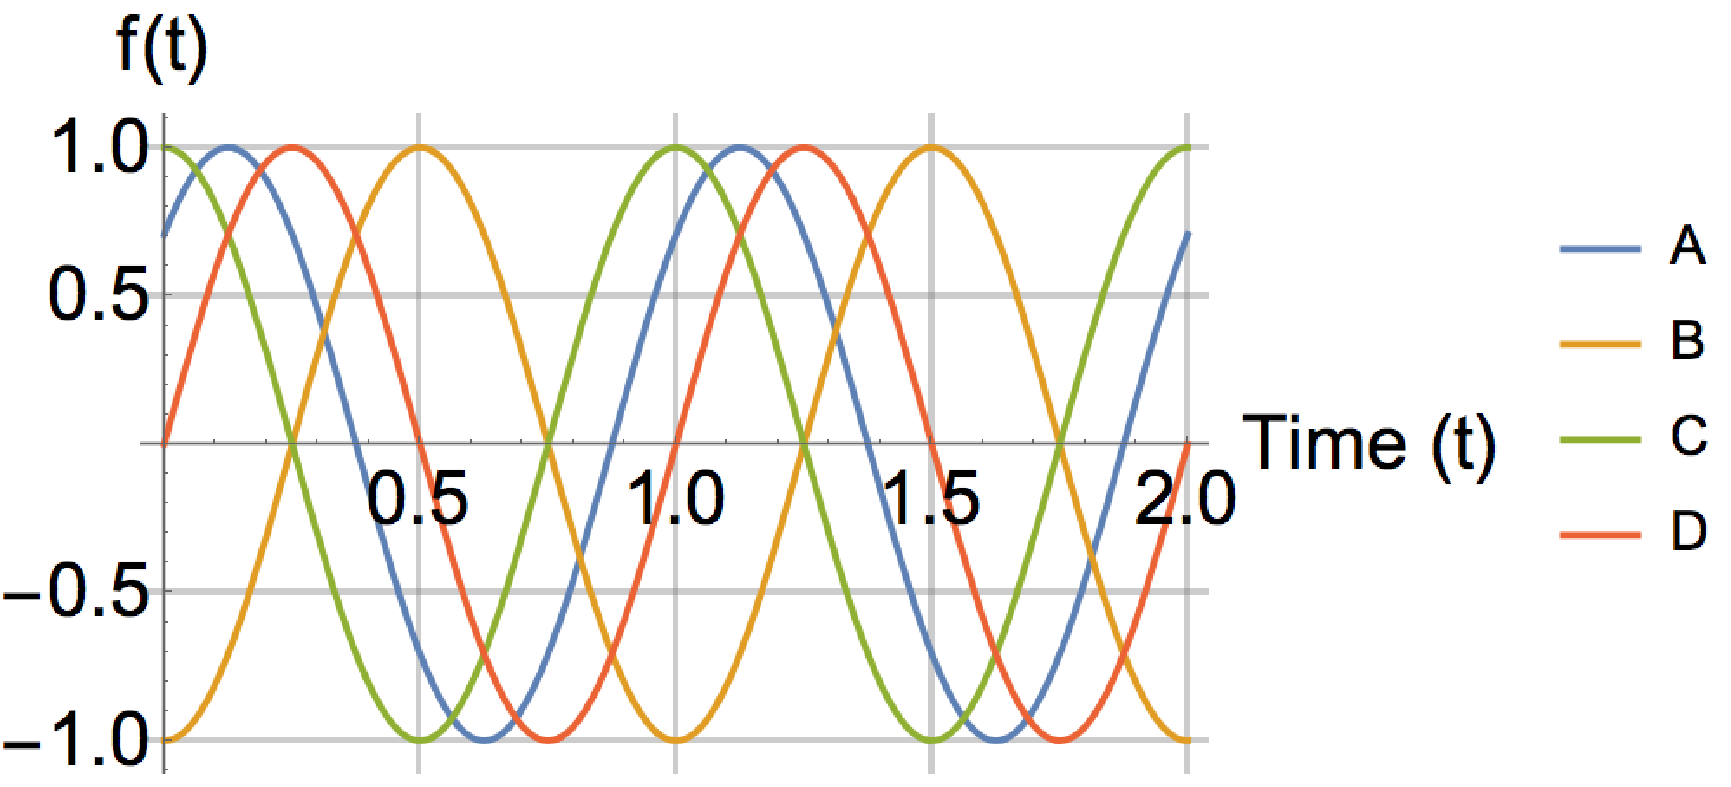
\includegraphics{phase_shift.png}

\subsection*{Solution}
\solstr{i}{5c0e8b}



%%%%%%%%%%%%%%%%%%%%%%%%%%%%%%%%%
\newpage
%%%%%%%%%%%%%%%%%%%%%%%%%%%%%%%%%
\section{Amplitude}

\subsection*{Comments}
Another important concept is amplitude. $\sin(2 \pi t)$ has an amplitude of 1, but this can be easily modified to go between $\pm A$ by multiplication with $A$.

\subsection*{Challenge}
The following 4 graphs correspond to the equation $A \sin(2 \pi k t)$ with variation in the values of $A$ and $k$. What is the sum of the values of $A$ for the following graphs? 

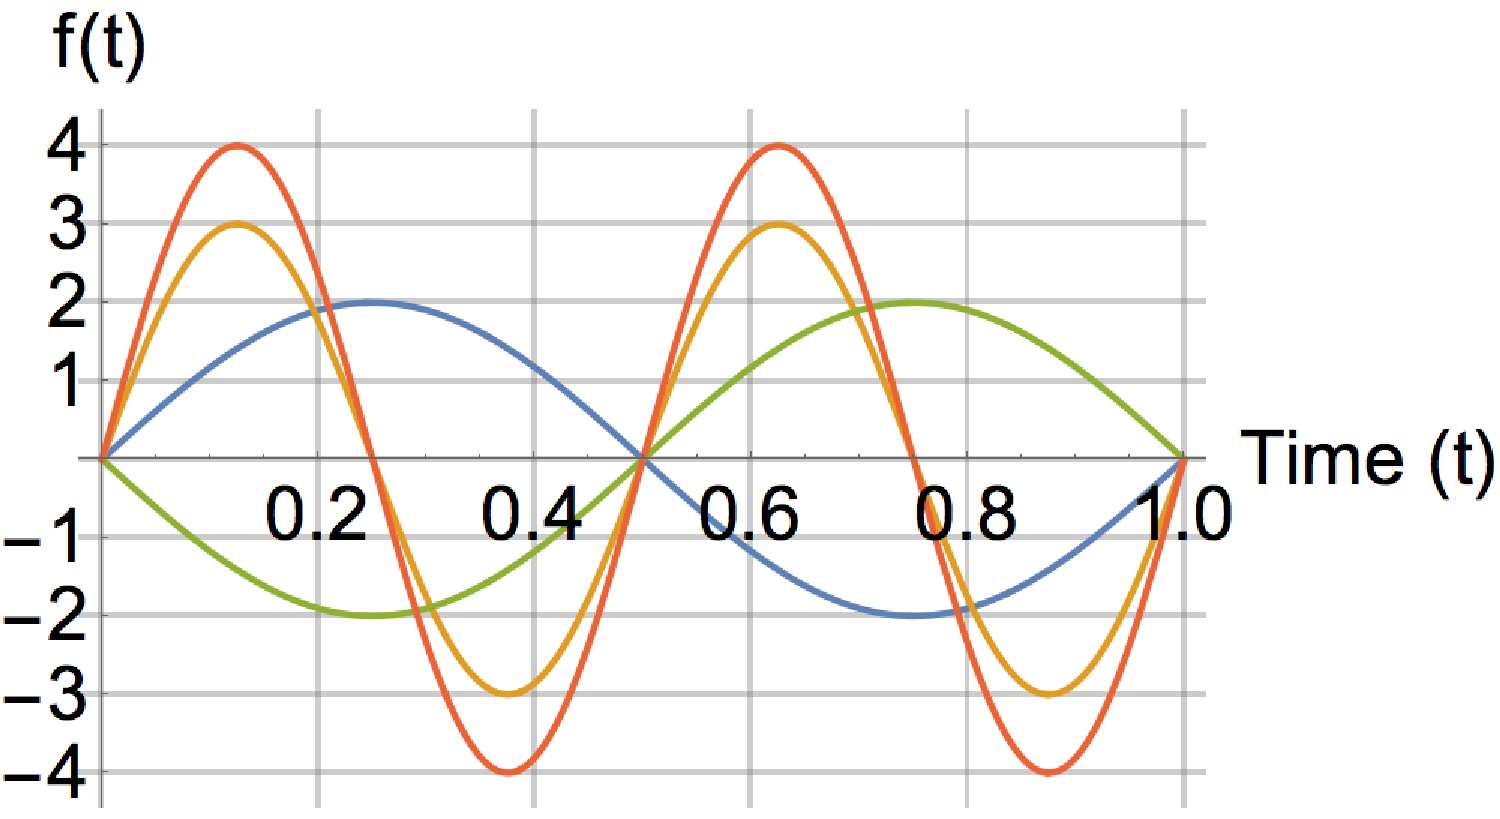
\includegraphics{amplitude.png}

\subsection*{Solution}
\solint{u}{6bce05}




%%%%%%%%%%%%%%%%%%%%%%%%%%%%%%%%%
\newpage
%%%%%%%%%%%%%%%%%%%%%%%%%%%%%%%%%
\section{Periodic and non-periodic signals}
\label{sec:periodic}

\subsection*{Resources}
\begin{itemize}
    \item Video: \url{https://www.youtube.com/watch?v=F_pdpbu8bgA}
    \item Book: 1.3 (\url{https://see.stanford.edu/materials/lsoftaee261/book-fall-07.pdf})
\end{itemize}

\subsection*{Challenge}
The list below contains periodic and non-periodic signals. Sum the points of the signals below that are \emph{periodic}.

1 point: $x(t) = t^2$\\
2 points: $x(t) = \sin(t)$\\
4 points: $x(t) = \sin(2 \pi t)$\\
8 points: $x(t) = \sin(2 \pi t + t)$\\
16 points: $x(t) = \sin(2 \pi t) + \sin(t)$\\
32 points: $x(t) = \sin(5 \pi t) + \sin(2 \pi t)$\\
64 points: $x(t) = \sin(5 \pi t) + \sin(37 \pi t)$\\
128 points: $x(t) = \sin(5 \pi t) + \sin(37.01 \pi t)$\\
256 points: $x(t) = \sin(5 \pi t) + \sin(\sqrt{2} \pi t)$\\
512 points: $x(t) = \sin(5 \sqrt{2} \pi t) + \sin(\sqrt{2} \pi t)$

\subsection*{Solution}
\solint{u}{5d906b}




%%%%%%%%%%%%%%%%%%%%%%%%%%%%%%%%%
\newpage
%%%%%%%%%%%%%%%%%%%%%%%%%%%%%%%%%
\section{Making non-periodic signals from periodic signals}

\subsection*{Challenge}
It is not immediately intuitive that it is possible to make a non-periodic signal by simply adding two periodic signals. Referring to the previous challenge, in no-more than 1 paragraph, explain how this is possible.

\subsection*{Solution}
Please compare your answer with your partner or ask the teacher in class.




%%%%%%%%%%%%%%%%%%%%%%%%%%%%%%%%%
\newpage
%%%%%%%%%%%%%%%%%%%%%%%%%%%%%%%%%
\section{Fundamental frequency}

\subsection*{Challenge}
Considering the periodic signals in challenge \ref{sec:periodic} in order of increasing point-score, calculate the fundamental frequency and period of the last periodic signal in the list.

\subsection*{Solution}
Frequency (Hz) (be careful about rounding up or down to 2 decimal places):\\
\soltwodp{a}{ac6698}

Period (s):\\
\soltwodp{b}{6fdff9}
